\clearpage
\subsubsectionold{\Optimizing MSVC + \olly}
\myindex{\olly}

Можем попробовать этот (соптимизированный) пример в \olly.  Вот самая первая итерация:

\begin{figure}[H]
\centering
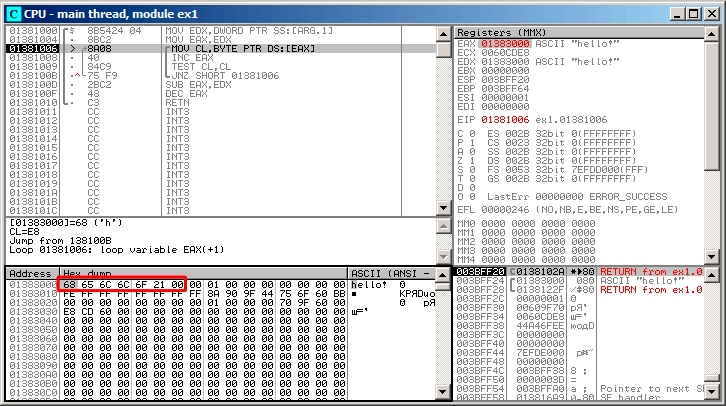
\includegraphics[scale=\FigScale]{patterns/10_strings/1_strlen/olly1.png}
\caption{\olly: начало первой итерации}
\label{fig:strlen_olly_1}
\end{figure}

Видно, что \olly обнаружил цикл и, для удобства, \IT{свернул} инструкции тела цикла в скобке.

Нажав правой кнопкой на \EAX, можно выбрать \q{Follow in Dump} 
и позиция в окне памяти будет как раз там, где надо.

Здесь мы видим в памяти строку \q{hello!}.
После неё имеется как минимум 1 нулевой байт, затем случайный мусор.
Если \olly видит, что в регистре содержится адрес какой-то строки, он показывает эту строку.

\clearpage
Нажмем F8 (\stepover) столько раз, чтобы текущий адрес снова был в начале тела цикла:

\begin{figure}[H]
\centering
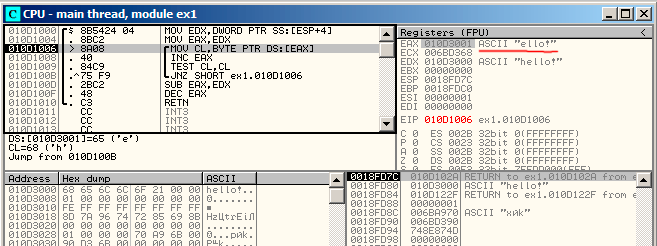
\includegraphics[scale=\FigScale]{patterns/10_strings/1_strlen/olly2.png}
\caption{\olly: начало второй итерации}
\label{fig:strlen_olly_2}
\end{figure}

Видно, что \EAX уже содержит адрес второго символа в строке.

\clearpage
Будем нажимать F8 достаточное количество раз, чтобы выйти из цикла:

\begin{figure}[H]
\centering
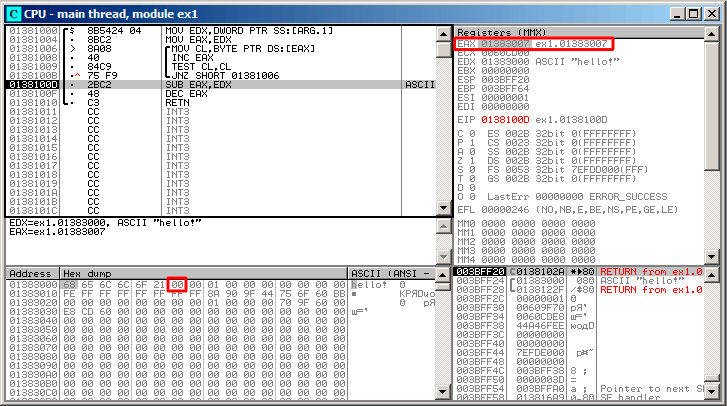
\includegraphics[scale=\FigScale]{patterns/10_strings/1_strlen/olly3.png}
\caption{\olly: сейчас будет вычисление разницы указателей}
\label{fig:strlen_olly_3}
\end{figure}

Увидим, что \EAX теперь содержит адрес нулевого байта, следующего сразу за строкой.

А \EDX так и не менялся~--- он всё ещё указывает на начало строки.
Здесь сейчас будет вычисляться разница между этими двумя адресами.

\clearpage
Инструкция \SUB исполнилась:

\begin{figure}[H]
\centering
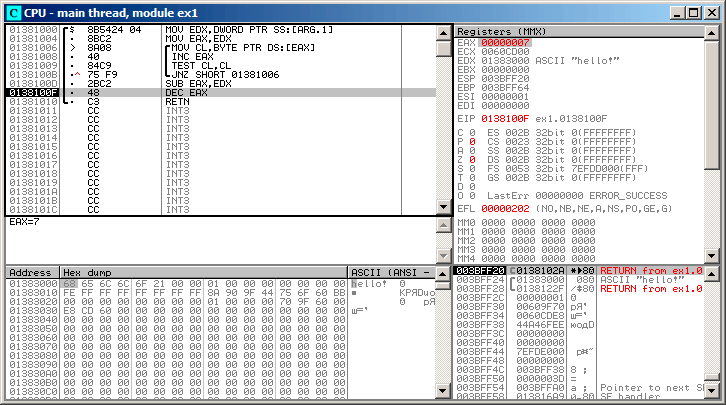
\includegraphics[scale=\FigScale]{patterns/10_strings/1_strlen/olly4.png}
\caption{\olly: сейчас будет декремент \EAX}
\label{fig:strlen_olly_4}
\end{figure}

Разница указателей сейчас в регистре \EAX~--- 7.

Действительно, длина строки \q{hello!}~--- 6, 
но вместе с нулевым байтом\EMDASH{}7.
Но \TT{strlen()} должна возвращать количество ненулевых символов в строке.
Так что сейчас будет исполняться декремент и выход из функции.

